\documentclass[12pt,a4paper]{article}

\usepackage[utf8]{inputenc}
\usepackage[T2A]{fontenc}
\usepackage[ukrainian]{babel}
\usepackage{geometry}
\geometry{
    left=2cm,
    right=2cm,
    top=2cm,
    bottom=2cm
}

\usepackage[table]{xcolor}
\usepackage{amsmath}
\usepackage{graphicx}
\usepackage{subcaption}
\usepackage{multirow}
\usepackage{makecell}
\usepackage{pdflscape}
\usepackage{array}
\newcolumntype{C}[1]{>{\centering\arraybackslash}m{#1}}

\usepackage[
  unicode,
  pdftitle={ІО-41, Давидчук А.М., Цифрова схемотехніка, Лабораторна робота №2},
  pdfauthor={Давидчук Артем},
  pdfsubject={Цифрова схемотехніка}
]{hyperref}

\begin{document}

    \begin{titlepage}

        \begin{center}
\includegraphics[width=0.7\textwidth]{../../../TITLES/letterhead.png}\end{center}

        \begin{center}
            \large Національний технічний університет України\\
            «Київський політехнічний інститут імені Ігоря Сікорського»\\[1em]
            Факультет інформатики та обчислювальної техніки\\
            Кафедра обчислювальної техніки
        \end{center}

        \vfill

        \begin{center}
            \textbf{\LARGE Цифрова схемотехніка}\\[2em]
            \textbf{\Large Лабораторна робота №2}\\[0.5em]
            «Суматори» 
        \end{center}

        \vfill

        \begin{flushright}
            Виконав: студент 2 курсу ФІОТ, гр. ІО-41\\
            \textit{Давидчук А. М.}\\
            Залікова книжка № 4106\\[1em]
            Перевірив: \textit{Нікольський С.\,С.}
        \end{flushright}

        \vfill

        \begin{center}Київ --- 2026\end{center}

    \end{titlepage}

    \noindent
    \textbf{\underline{Тема:}} «Суматори».

    \vspace{1em}

    \begin{center} \textbf{\Large Хід роботи} \end{center}

    Мій номер залікової книжки: 4106, що у двіковому вигляді є 0001 0000 0000 1010.
    Звідси $h_7 = 0, h_6 = 0, h_5 = 0, h_4 = 1, h_3 = 0, h_2 = 1, h_1 = 0$. Звідси маю такий варіант:

    \begin{table}[h!]
        \centering
        \renewcommand{\arraystretch}{1.3}
        \begin{tabular}{|c|c|}
            \hline
            \textbf{Номер варіанта} & \textbf{Розрядність суматора} \\ \hline
            0\hspace{1em}0\hspace{1em}0 & 16 \\ \hline
            0\hspace{1em}0\hspace{1em}1 & 15 \\ \hline
            \rowcolor{yellow!50}
            0\hspace{1em}1\hspace{1em}0 & 14 \\ \hline
            0\hspace{1em}1\hspace{1em}1 & 12 \\ \hline
            1\hspace{1em}0\hspace{1em}0 & 11 \\ \hline
            1\hspace{1em}0\hspace{1em}1 & 10 \\ \hline
            1\hspace{1em}1\hspace{1em}0 & 9  \\ \hline
            1\hspace{1em}1\hspace{1em}1 & 8  \\ \hline
        \end{tabular}
    \end{table}

    \begin{table}[h!]
        \centering
        \renewcommand{\arraystretch}{1.3}
        \begin{tabular}{|c|c|}
            \hline
            \textbf{Номер групи} & \textbf{Розряди номера ЗК} \\ \hline
            \rowcolor{yellow!50}
            IX-*1 & $h_1 \; h_2 \; h_3$ \\ \hline
            IX-*2 & $h_3 \; h_2 \; h_1$ \\ \hline
            IX-*3 & $h_2 \; h_4 \; h_1$ \\ \hline
            IX-*4 & $h_3 \; h_1 \; h_2$ \\ \hline
            IX-*5 & $h_4 \; h_2 \; h_3$ \\ \hline
            IX-*6 & $h_4 \; h_2 \; h_1$ \\ \hline
        \end{tabular}
    \end{table}

    \newpage

    \begin{center} \textbf{\large Версія v1 проекту} \end{center}

    В цій версії ми будемо реалізувати однорозрядний суматор за допомогою одного вручну побудованого напівсуматора, та готового напівсуматора в \textbf{MegaWizard Plug-in Manager}.

    \begin{figure}[h]
        \centering
        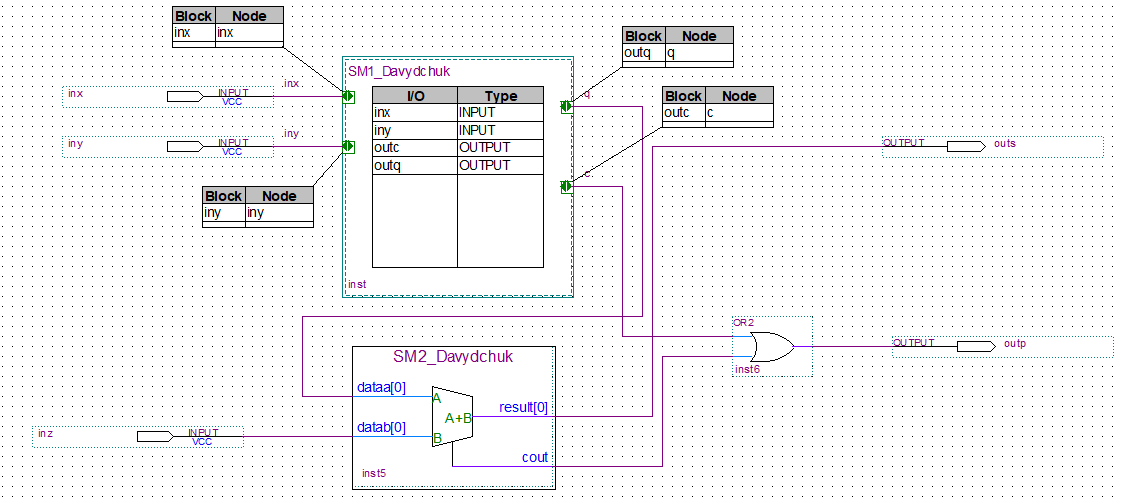
\includegraphics[width=0.8\textwidth]{media/image0.png}
        \caption{Верхній рівень реалізації однорозрядного суматора}
    \end{figure}

    \begin{figure}[h]
        \centering
        
\includegraphics[width=0.8\textwidth]{media/image1.png}
        \caption{Функціональна схема напівсуматора}
    \end{figure}

    \noindent
    Тепер проведемо компіляцію та зафіксуємо результати:

    \begin{figure}[h]
        \centering
        
\includegraphics[width=0.8\textwidth]{media/image2.png}
    \end{figure}

    \newpage

    \begin{figure}[h]
        \centering
        
\includegraphics[width=0.8\textwidth]{media/image3.png}
    \end{figure}

    \begin{figure}[h]
        \centering
        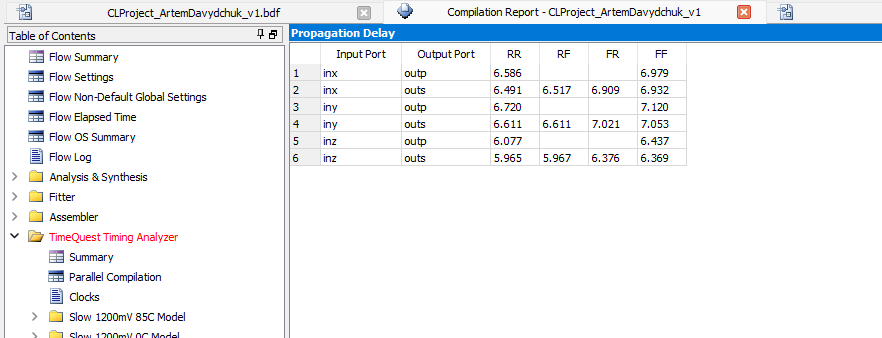
\includegraphics[width=0.8\textwidth]{media/image4.png}
        \caption{Результати компіляції першої версії проекту}
    \end{figure}

    \begin{center} \textbf{\large Версія v2 проекту} \end{center}

    В цій версії ми будемо реалізувати однорозрядний суматор за допомогою \textbf{MegaWizard Plug-in Manager}.

    \begin{figure}[h]
        \centering
        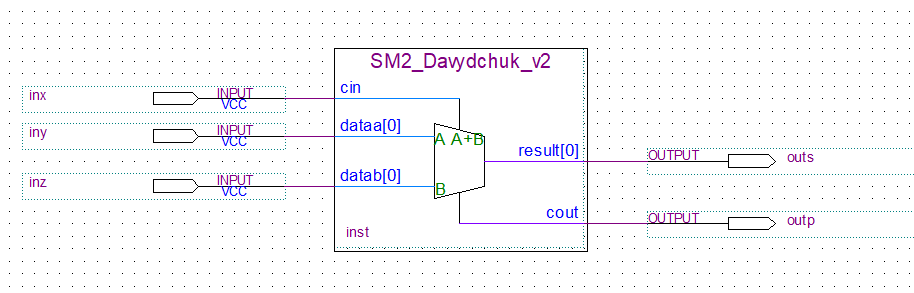
\includegraphics[width=0.8\textwidth]{media/image5.png}
        \caption{Схема однорозрядного суматора}
    \end{figure}

    \newpage

    \noindent
    І знову проведемо компіляцію та зафіксуємо результати:

    \begin{figure}[h]
        \centering
        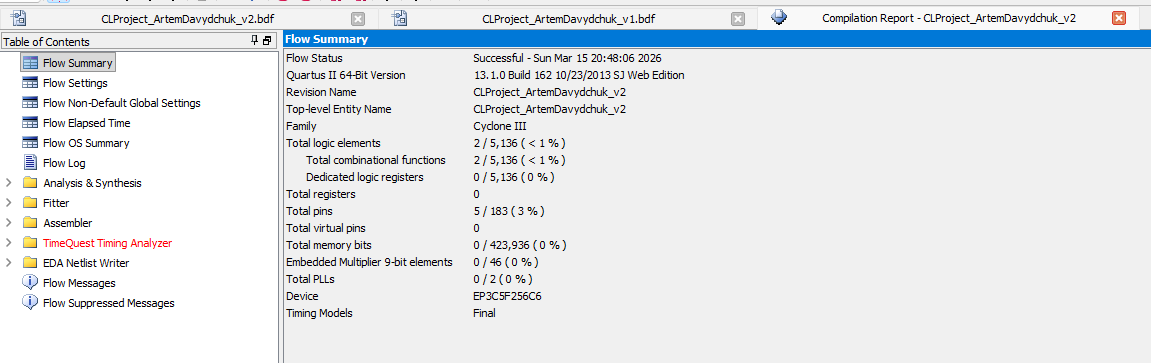
\includegraphics[width=0.8\textwidth]{media/image6.png}
    \end{figure}

    \begin{figure}[h]
        \centering
        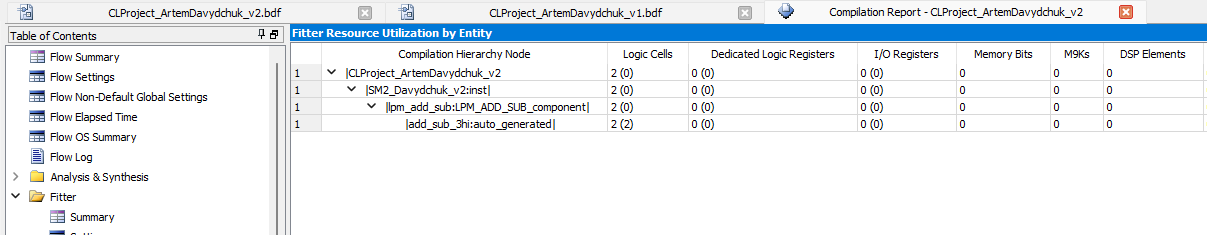
\includegraphics[width=0.8\textwidth]{media/image7.png}
    \end{figure}

    \begin{figure}[h]
        \centering
        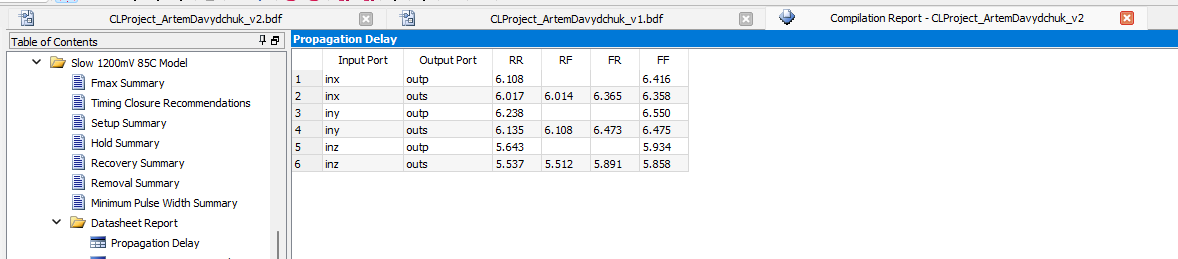
\includegraphics[width=0.8\textwidth]{media/image8.png}
        \caption{Результати компіляції другої версії проекту}
    \end{figure}

    \noindent
    Тепер підведемо підсумки компіляцій обох проектів в одну таблицю:

    \begin{table}[h!]
        \centering
        \footnotesize
        \renewcommand{\arraystretch}{1.2}
        
        \newcolumntype{C}[1]{>{\centering\arraybackslash}p{#1}}
        
        \begin{tabular}{|C{4.6cm}|C{5.5cm}|C{5.5cm}|}
            \hline
            \textbf{Звіти компілятора} &
            \makecell{\textbf{CLProject\_ArtemDavydchuk\_}\\\textbf{v1}} &
            \makecell{\textbf{CLProject\_ArtemDavydchuk\_}\\\textbf{v2}}
            \\ \hline

            Total logic elements &
            2 / 5,136 ($< 1 \%$) &
            2 / 5,136 ($< 1 \%$)
            \\ \hline

            Total combinational functions &
            2 / 5,136 ($< 1 \%$) &
            2 / 5,136 ($< 1 \%$)
            \\ \hline

            Dedicated logic registers &
            0 / 5,136 ($0 \%$) &
            0 / 5,136 ($0 \%$)
            \\ \hline

            Total registers &
            0 &
            0
            \\ \hline

            Total pins &
            5 / 183 ($3 \%$) &
            5 / 183 ($3 \%$)
            \\ \hline

            Total virtual pins &
            0 &
            0
            \\ \hline

            Total memory bits &
            0 / 423,936 ($0 \%$) &
            0 / 423,936 ($0 \%$)
            \\ \hline

            Embedded multiplier 9-bit elements &
            0 / 46 ($0 \%$) &
            0 / 46 ($0 \%$)
            \\ \hline

            Total PPLs &
            0 / 2 ($0 \%$) &
            0 / 2 ($0 \%$)
            \\ \hline
        \end{tabular}
    \end{table}

    \newpage

    \begin{center} \textbf{\large Логічна реалізація схеми} \end{center}

    \begin{figure}[h]
        \centering
        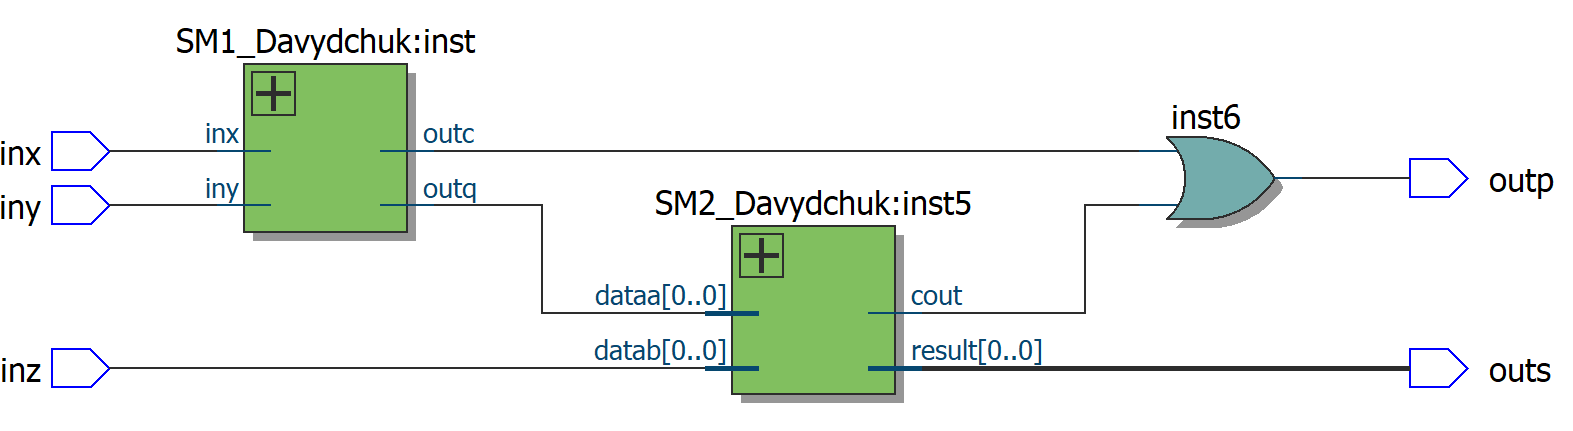
\includegraphics[width=\textwidth]{media/image9.png}
        \caption{Логічна реалізація першої версії проекту}
    \end{figure}

    \begin{figure}[h]
        \centering
        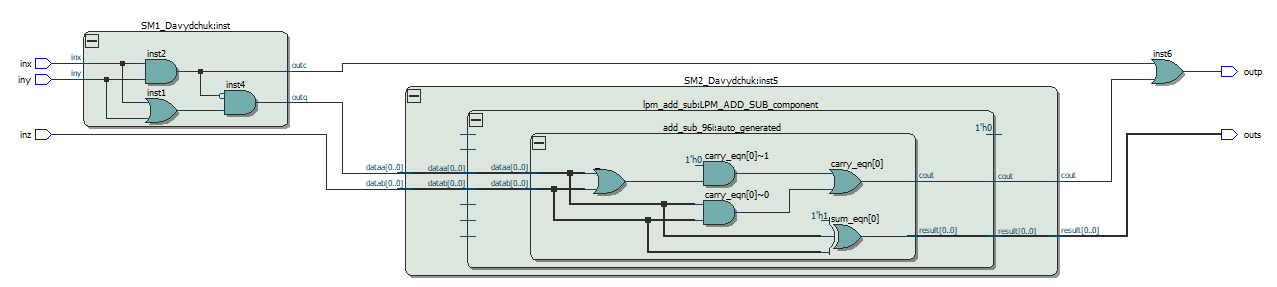
\includegraphics[width=\textwidth]{media/image10.png}
        \caption{Логічна структура реалізації блоків та загальної схеми}
    \end{figure}

    \newpage

    \begin{figure}[h]
        \centering
        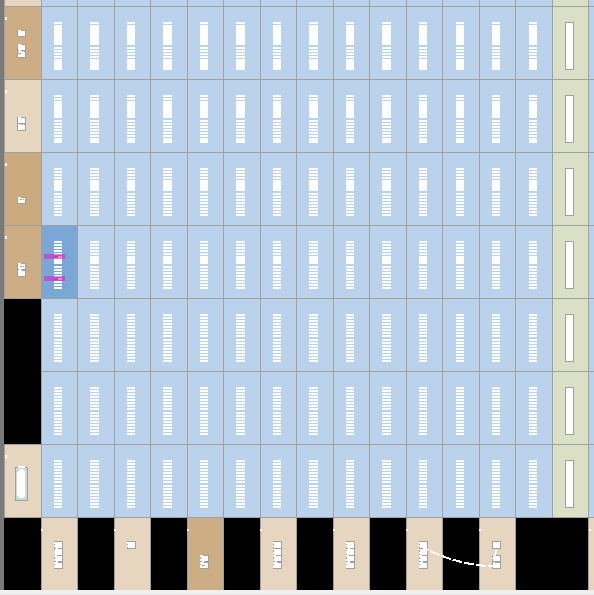
\includegraphics[width=0.9\textwidth]{media/image11.png}
        \caption{Розміщення логічних ресурсів на мікросхемі \textbf{Cyclon III}.}
    \end{figure}

    \newpage

    \begin{figure}[h]
        \centering
        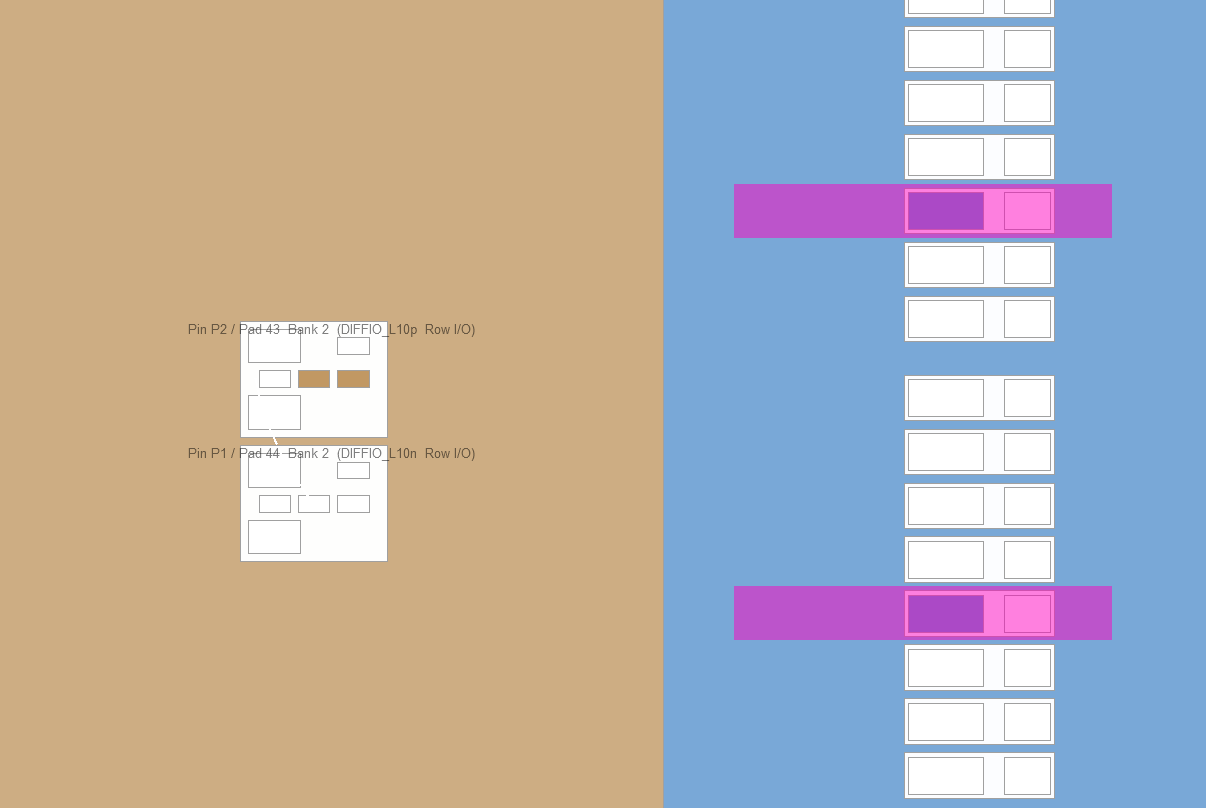
\includegraphics[width=0.9\textwidth]{media/image12.png}
        \caption{Збільшений фрагмент кристалу у редакторі Chip Planner}
    \end{figure}

    \begin{figure}[h]
        \centering
        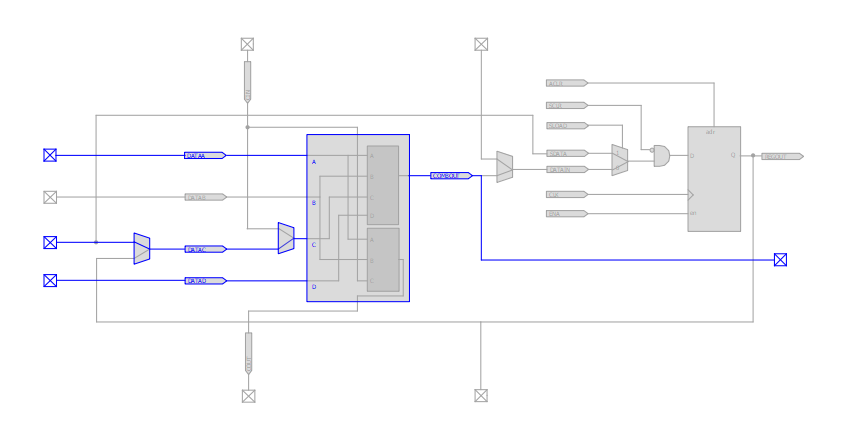
\includegraphics[width=0.8\textwidth]{media/image13.png}
    \end{figure}

    \newpage

    \begin{figure}[h]
        \centering
        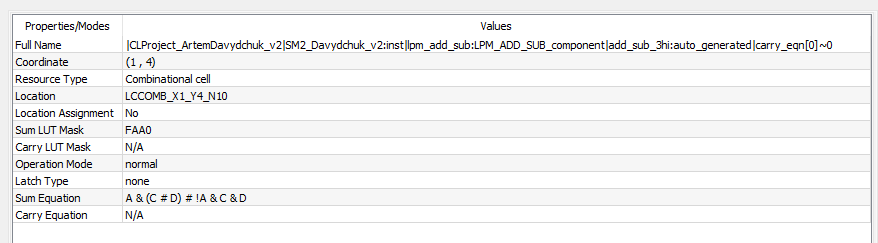
\includegraphics[width=0.8\textwidth]{media/image14.png}
    \end{figure}

    \begin{figure}[h]
        \centering
        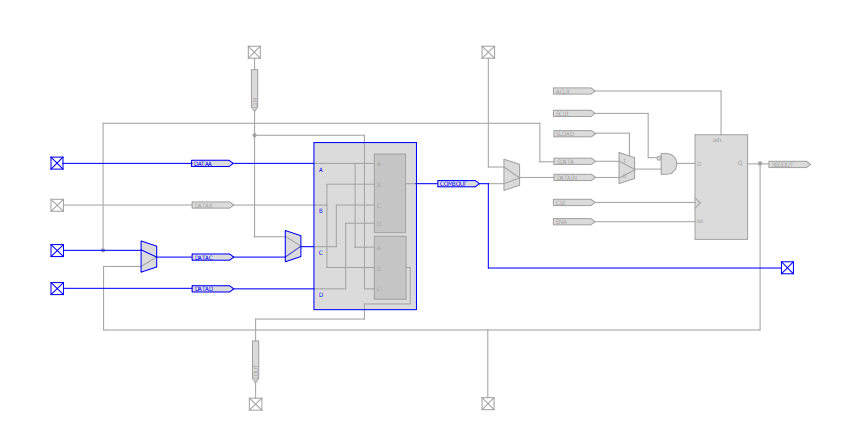
\includegraphics[width=0.8\textwidth]{media/image15.png}
    \end{figure}

    \begin{figure}[h]
        \centering
        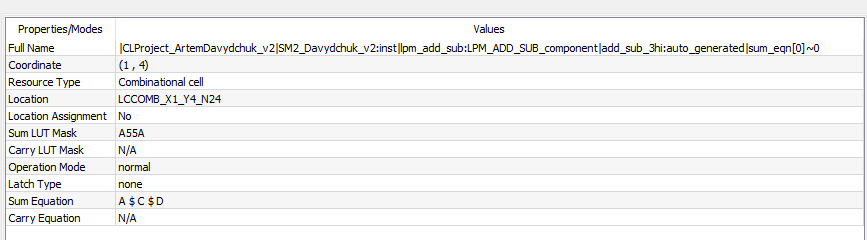
\includegraphics[width=0.8\textwidth]{media/image16.png}
        \caption{Аналіз використаних ресурсів логічних комірок}
    \end{figure}

    \newpage

    \begin{center} \textbf{\large Створення 14-розрядного суматора} \end{center}

    Тепер за варіантом нам потрібно створити 140розрядного суматора на основі вже готового однорозрядного суматора із \textbf{MegaWizard Plug-in Manager}.

    \begin{figure}[h]
        \centering
        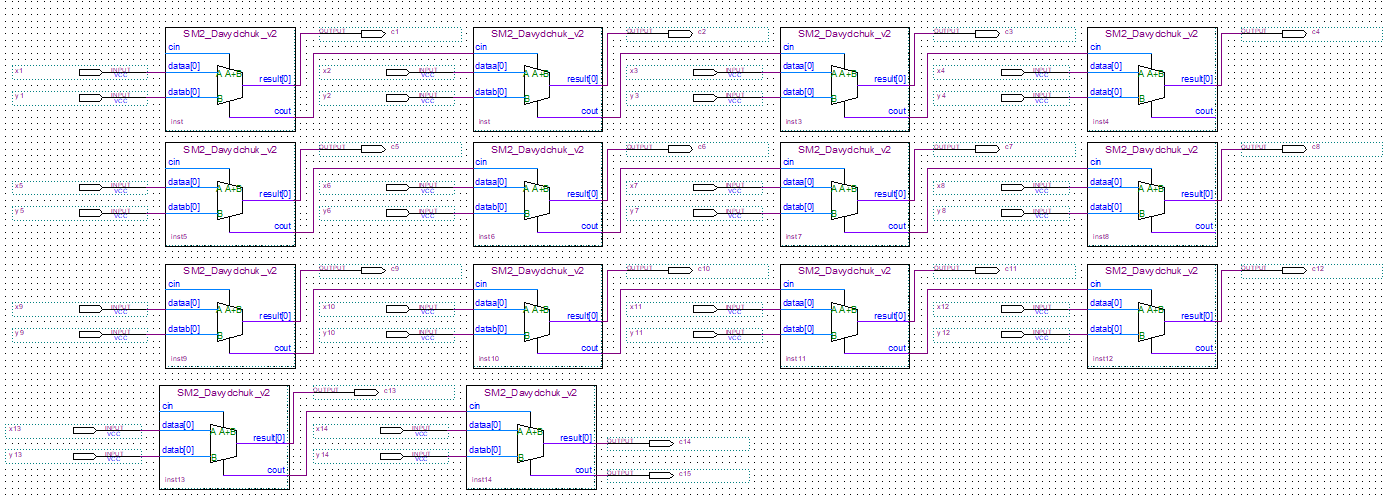
\includegraphics[width=\textwidth]{media/image17.png}
        \caption{Реалізована схема 14-розрядного суматора}
    \end{figure}

    Та проведемо компіляцію та зафіксуємо результати:

    \begin{figure}[h]
        \centering
        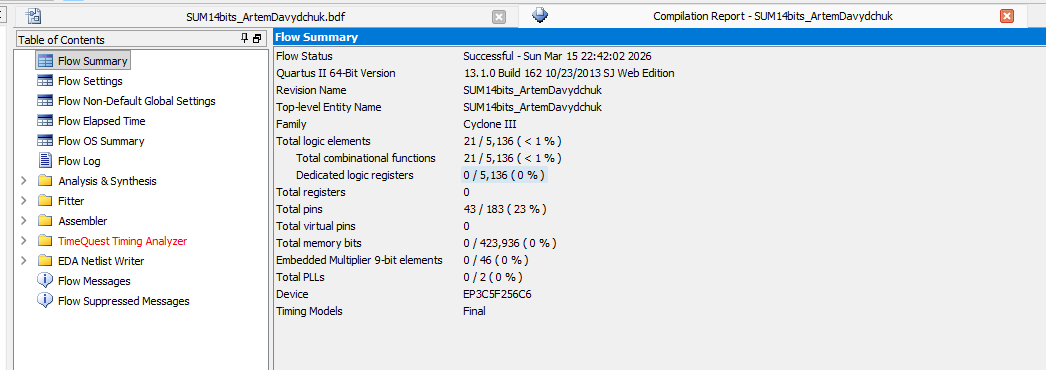
\includegraphics[width=0.8\textwidth]{media/image18.png}
    \end{figure}

    \begin{figure}[h]
        \centering
        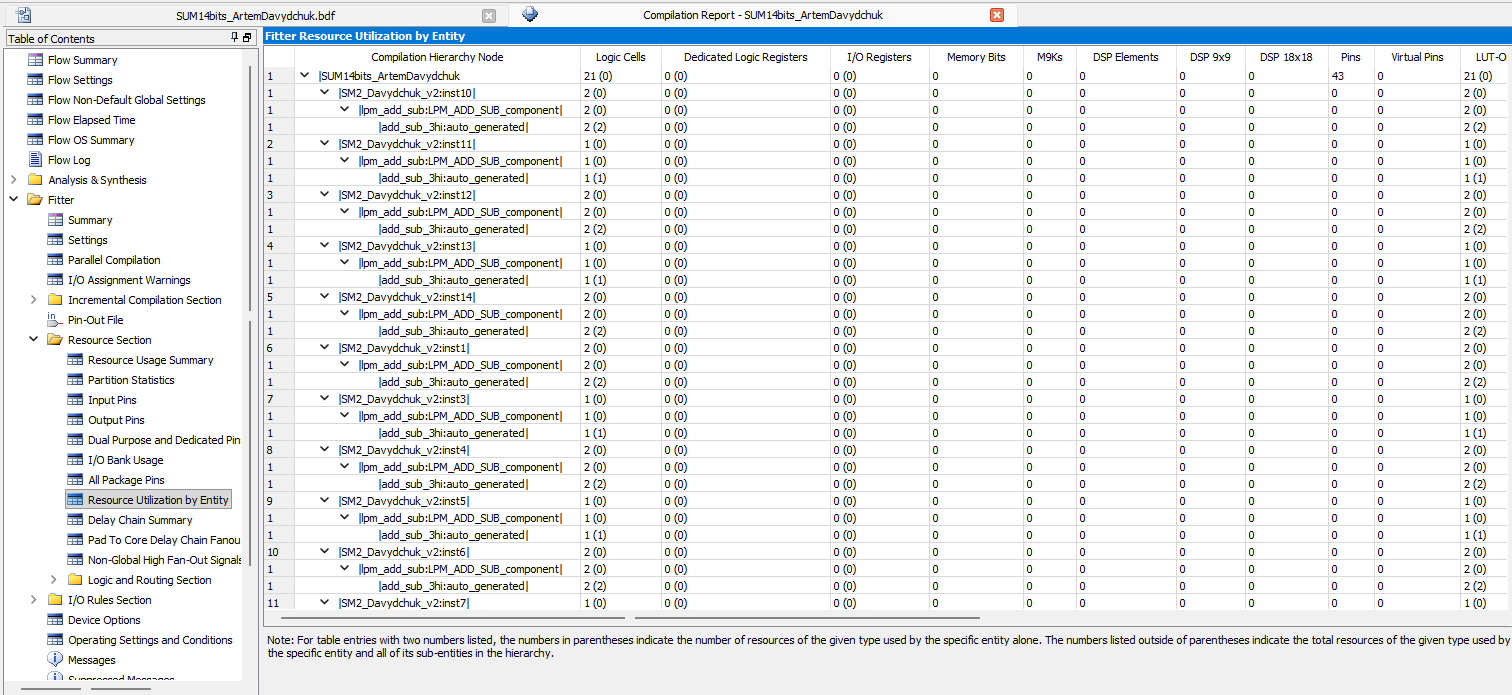
\includegraphics[width=0.8\textwidth]{media/image19.png}
    \end{figure}

    \newpage

    \begin{figure}[h]
        \centering
        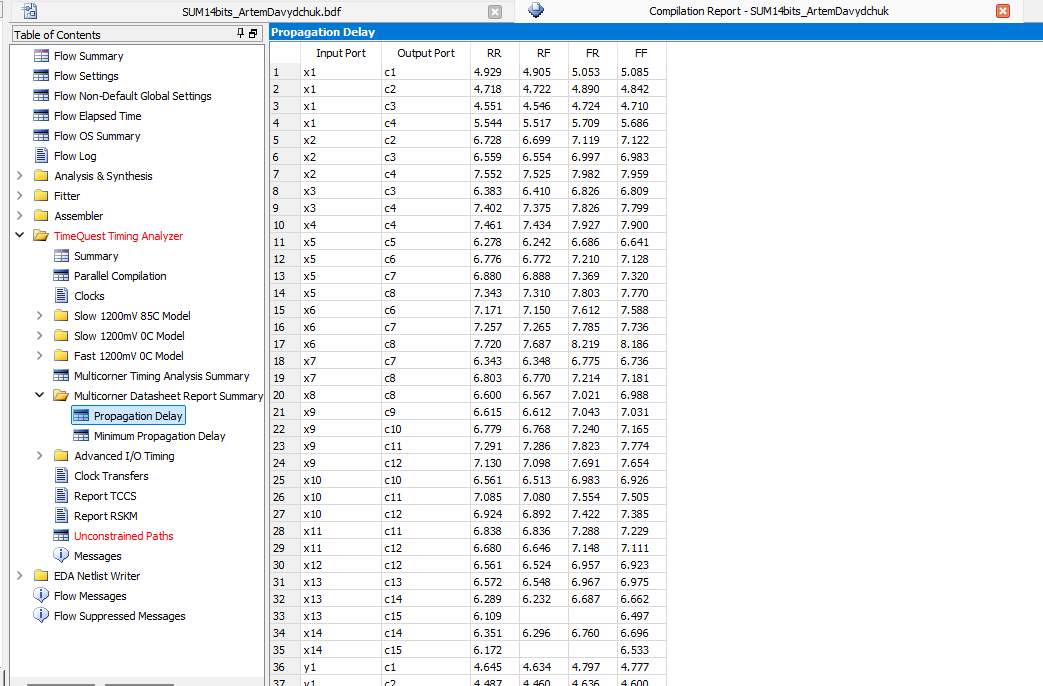
\includegraphics[width=0.8\textwidth]{media/image20.png}
        \caption{Аналіз звіту компіляції 14-розрядного суматора}
    \end{figure}

    \begin{figure}[h]
        \centering
        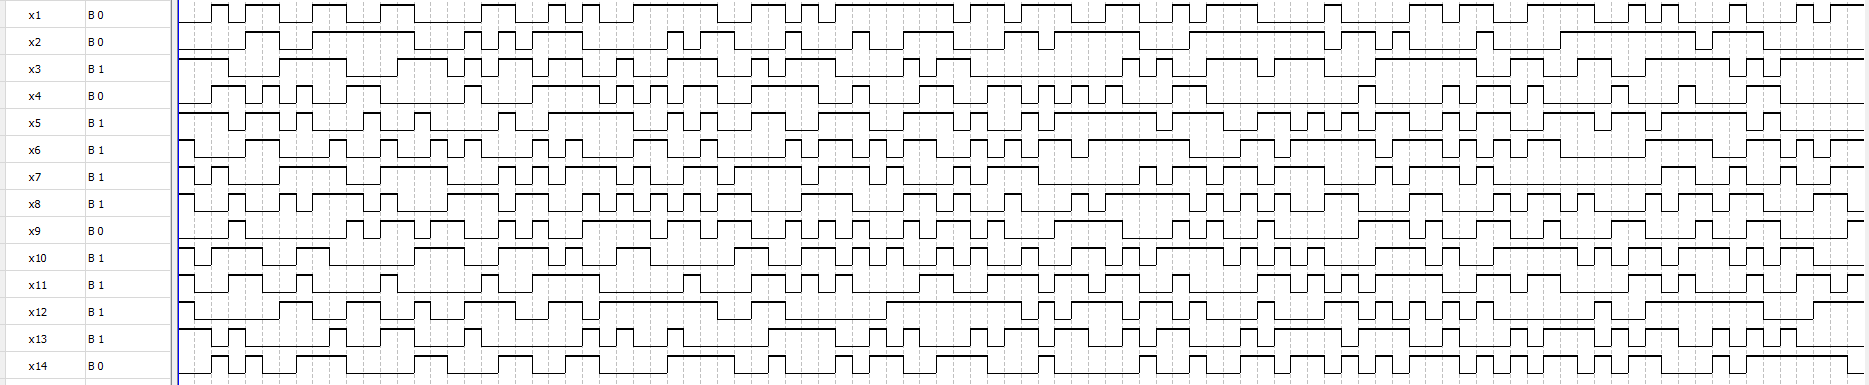
\includegraphics[width=\textwidth]{media/image21.png}
    \end{figure}

    \begin{figure}[h]
        \centering
        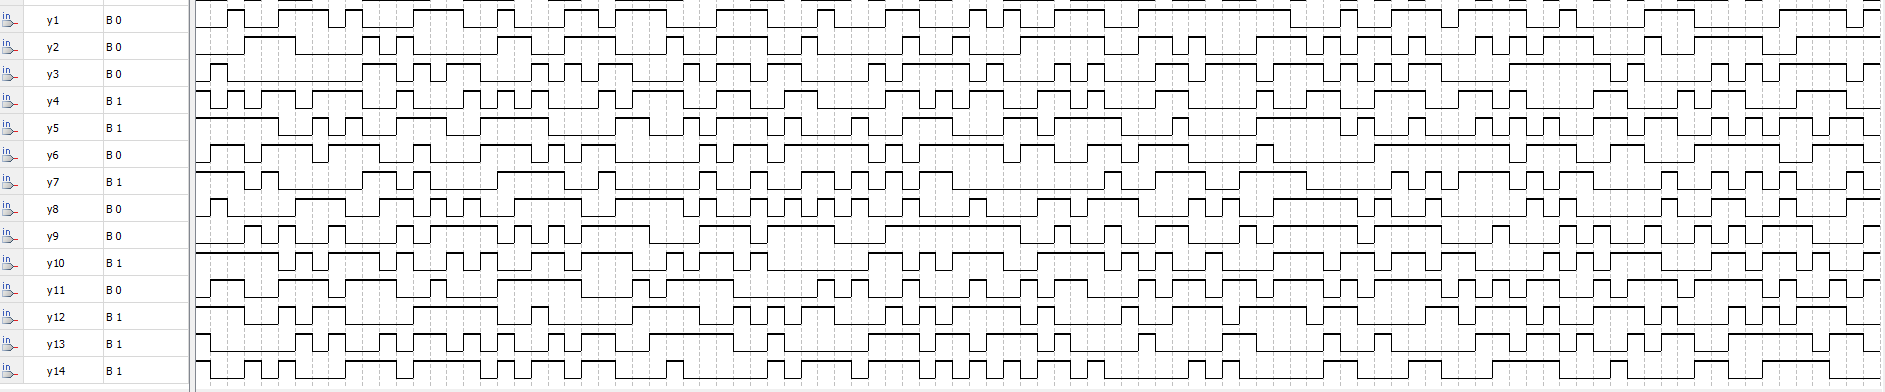
\includegraphics[width=\textwidth]{media/image22.png}
    \end{figure}

    \newpage

    \begin{figure}[h]
        \centering
        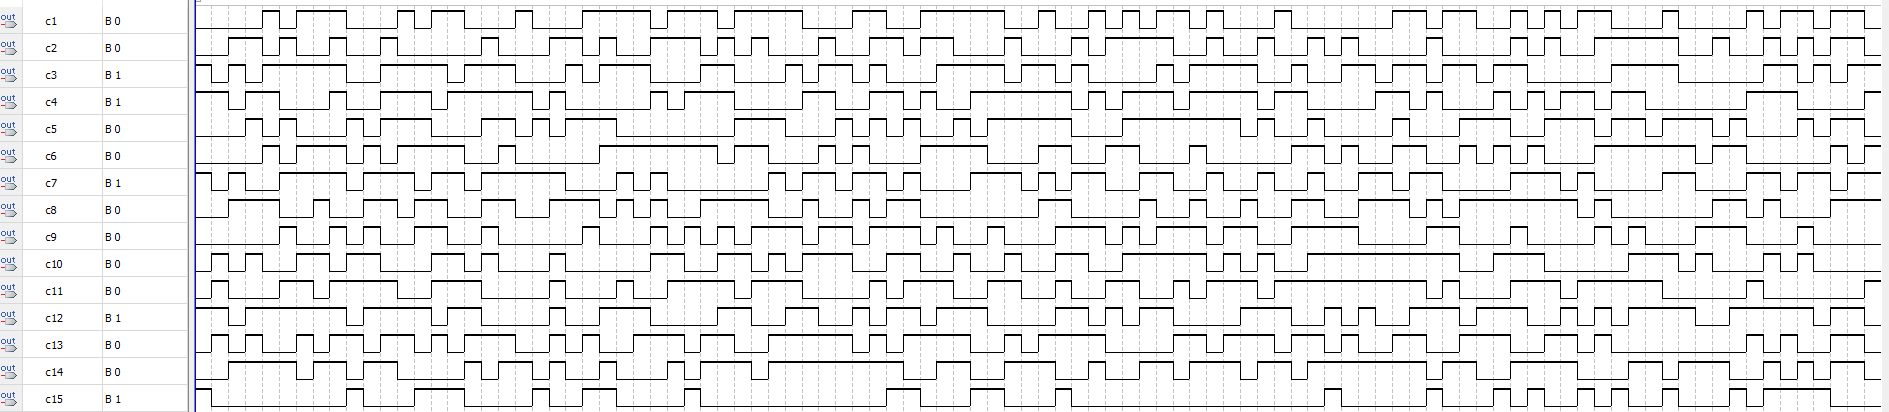
\includegraphics[width=\textwidth]{media/image23.png}
        \caption{Аналіз зміни вхідних та вихідних сигналів під час симуляції}
    \end{figure}

    \begin{center} \textbf{\Large Висновок} \end{center}

    Під час виконання лабораторної роботи було реалізовано та досліджено схеми однорозрядного і багаторозрядного суматорів у середовищі Quartus II. Було побудовано дві версії однорозрядного суматора: першу --- з використанням вручну створеного напівсуматора та готового модуля, другу --- із застосуванням засобів \textbf{MegaWizard Plug-in Manager}. Для обох реалізацій проведено компіляцію, аналіз звітів та дослідження логічної структури схеми.

    За допомогою засобів RTL Viewer, Technology Map Viewer і Chip Planner було проаналізовано особливості логічної реалізації проєкту, використання ресурсів мікросхеми та розміщення елементів на кристалі. Результати компіляції показали, що обидва варіанти однорозрядного суматора мають однакові показники використання апаратних ресурсів.

    На основі однорозрядного суматора було синтезовано 14-розрядний суматор відповідно до індивідуального варіанту. Проведене моделювання підтвердило коректність його функціонування. Отже, у ході роботи було отримано практичні навички побудови суматорів, аналізу результатів синтезу та дослідження апаратної реалізації цифрових схем у ПЛІС.

\end{document}